%%%%%%%%%%%%%%%%%%%%%%%%%%%%%%%%%%%%%%%%%%%%%%%%%%%%%%%%%%%%%%%%%%%%%%%%
% Escuela Politécnica Superior de la Universidad de Alicante
% Realizado por: Jose Manuel Requena Plens
% Contacto: info@jmrplens.com / Telegram:@jmrplens
%%%%%%%%%%%%%%%%%%%%%%%%%%%%%%%%%%%%%%%%%%%%%%%%%%%%%%%%%%%%%%%%%%%%%%%%

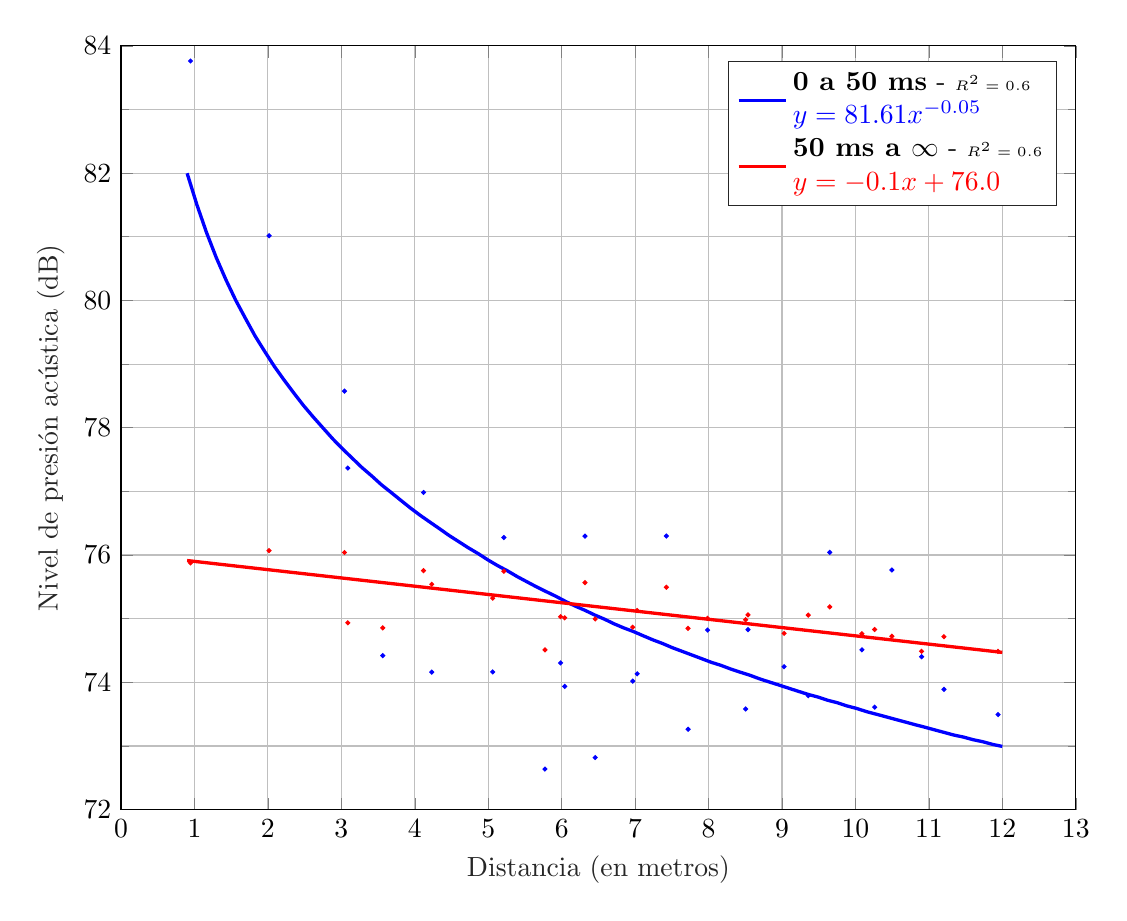
\begin{tikzpicture}

\begin{axis}[%
width=\textwidth,
height=0.8\textwidth,
at={(0\textwidth,0\textwidth)},
scale only axis,
xmin=0,
xmax=13,
xlabel style={font=\color{white!15!black}},
xlabel={Distancia (en metros)},
ymin=72,
ymax=84,
xmajorgrids,
xminorgrids,
ymajorgrids,
yminorgrids,
minor y tick num= 1,
ylabel style={font=\color{white!15!black}},
ylabel={Nivel de presión acústica (dB)},
axis background/.style={fill=white},
legend style={legend cell align=left, align=left, draw=white!15!black}
]
\addplot [color=blue, only marks,mark size=0.7pt, forget plot]
  table[row sep=crcr]{%
0.945832966226064	83.7613723273159\\
2.0155892438689	81.0162423459966\\
3.04292622322659	78.5741340871889\\
3.08781476128345	77.3661694070126\\
3.56407070636934	74.4195447651733\\
4.11885906532379	76.9825018479041\\
4.23076825174815	74.1614948370034\\
5.0601383380299	74.1635047432433\\
5.21338661524349	76.2742875281612\\
5.7725297747175	72.6376750158334\\
5.98493107729738	74.3045302985103\\
6.04070360140274	73.9359821507463\\
6.31685048105462	76.2962616688626\\
6.45653932071973	72.8184525162864\\
6.96725196903341	74.0197233913669\\
7.02797979507625	74.1332978831264\\
7.42526767194288	76.2979528676753\\
7.72055049850721	73.2624003422856\\
7.98590007450632	74.8209368605219\\
8.5047104595042	73.5815675022983\\
8.53670896774629	74.8278098704551\\
9.02858792946051	74.2461859060413\\
9.35746226281464	73.7897862980008\\
9.65012953280939	76.0413437836555\\
10.0878639959111	74.5098029500084\\
10.2617201287114	73.6092755871979\\
10.4960706933595	75.7646635864789\\
10.8998853204976	74.4019326738631\\
11.2050211958747	73.8894451766927\\
11.9413148354777	73.4937384336641\\
};
\addplot[color=blue,domain=0.9:12, samples=85,line width=1.2]{81.61*x^(-0.045)};
\addlegendentry{\textbf{0 a 50 ms} - \tiny{$R^2 = 0.6$}\\$\color{blue}y = 81.61·x^{-0.05}$}

\addplot [color=red, only marks,mark size=0.7pt, forget plot]
  table[row sep=crcr]{%
0.945832966226064	75.8756831712236\\
2.0155892438689	76.0688117402114\\
3.04292622322659	76.0395356654983\\
3.08781476128345	74.9352478473615\\
3.56407070636934	74.8553844312649\\
4.11885906532379	75.7543937944735\\
4.23076825174815	75.540482339615\\
5.0601383380299	75.3223520645197\\
5.21338661524349	75.7450970961607\\
5.7725297747175	74.5101521130851\\
5.98493107729738	75.0309510163013\\
6.04070360140274	75.0132759751214\\
6.31685048105462	75.5655547954218\\
6.45653932071973	74.9956410748914\\
6.96725196903341	74.8655502346388\\
7.02797979507625	75.1283568472655\\
7.42526767194288	75.4940077965527\\
7.72055049850721	74.8471381044347\\
7.98590007450632	75.004616004375\\
8.5047104595042	74.9841736554508\\
8.53670896774629	75.0586998621683\\
9.02858792946051	74.7687602281066\\
9.35746226281464	75.0566535033458\\
9.65012953280939	75.1842952487827\\
10.0878639959111	74.7630381678478\\
10.2617201287114	74.8297960943133\\
10.4960706933595	74.7247830880759\\
10.8998853204976	74.4871393636727\\
11.2050211958747	74.7165933582166\\
11.9413148354777	74.4864585207557\\
};
\addplot[color=red,domain=0.9:12, samples=85,line width=1.2]{-0.13*x+76.03};
\addlegendentry{\textbf{50 ms a $\infty$} - \tiny{$R^2 = 0.6$}\\$\color{red}y = -0.1·x+76.0$}

\end{axis}
\end{tikzpicture}%